%; whizzy chapter
% -initex iniptex -latex platex -format platex -bibtex jbibtex -fmt fmt
% $B0J>e(B whizzytex $B$r;HMQ$9$k>l9g$N@_Dj!#(B

%     Tokyo Debian Meeting resources
%     Copyright (C) 2010 Junichi Uekaw
%     Copyright (C) 2010 Nobuhiro Iwamatsu

%     This program is free software; you can redistribute it and/or modify
%     it under the terms of the GNU General Public License as published by
%     the Free Software Foundation; either version 2 of the License, or
%     (at your option) any later version.

%     This program is distributed in the hope that it will be useful,
%     but WITHOUT ANY WARRANTY; without even the implied warranty of
%     MERCHANTABILITY or FITNESS FOR A PARTICULAR PURPOSE.  See the
%     GNU General Public License for more details.

%     You should have received a copy of the GNU General Public License
%     along with this program; if not, write to the Free Software
%     Foundation, Inc., 51 Franklin St, Fifth Floor, Boston, MA  02110-1301 USA

%  preview (shell-command (concat "evince " (replace-regexp-in-string "tex$" "pdf"(buffer-file-name)) "&"))
% $B2hA|%U%!%$%k$r=hM}$9$k$?$a$K$O(Bebb$B$rMxMQ$7$F(Bboundingbox$B$r:n@.!#(B
%(shell-command "cd image201002; ebb *.png")

%%$B$3$3$+$i%X%C%@3+;O!#(B

\documentclass[mingoth,a4paper]{jsarticle}
\usepackage{monthlyreport}
\usepackage{wrapfig}

% $BF|IU$rDj5A$9$k!"Kh7nJQ$o$j$^$9!#(B
\newcommand{\debmtgyear}{2010}
\newcommand{\debmtgmonth}{4}
\newcommand{\debmtgdate}{17}
\newcommand{\debmtgnumber}{63}

\begin{document}

\begin{titlepage}
\thispagestyle{empty}

% $B%?%$%H%k%Z!<%8(B:$BJT=8I,MW$JItJ,$O:G=i$N%^%/%m$KHt$P$9$3$H(B

\vspace*{-2cm}
$BBh(B\debmtgnumber{}$B2s(B $BEl5~%(%j%"(B Debian $BJY6/2q;qNA(B\\
\hspace*{-2cm}
\includegraphics[width=210mm]{image201003/debsen.eps}\\
\hfill{}\debmtgyear{}$BG/(B\debmtgmonth{}$B7n(B\debmtgdate{}$BF|(B

\rotatebox{10}{\fontsize{32}{32} {\gt $BFC=8#1(B: piuparts$B$N;H$$J}(B}}

\rotatebox{10}{\fontsize{32}{32} {\gt $BFC=8#2(B: debtags$BF~Lg(B} }

\vspace*{-2cm}
\hfill{}
\includegraphics[height=6cm]{image200502/openlogo-nd.eps}
\end{titlepage}

\dancersection{Introduction}{$B>e@n(B $B=c0l(B}

\begin{multicols}{2}
 
 
 $B:#7n$N(BDebian$BJY6/2q$X$h$&$3$=!#$3$l$+$i(BDebian$B$N@$3&$K$"$7$rF'$_F~$l$k$H(B
 $B$$$&J}$b!"$9$G$K$I$C$W$j$H$D$+$C$F$$$k$H$$$&J}$b!"7n$K0l2s(BDebian$B$K$D$$(B
 $B$F8l$j$^$;$s$+!)(B

 Debian$BJY6/2q$NL\E*$O2<5-$G$9!#(B

 \begin{itemize}
 \item \underline{Debian Developer} ($B3+H/<T(B)$B$N0i@.!#(B
 \item $BF|K\8l$G$N!V(B\underline{$B3+H/$K4X$9$k>pJs(B}$B!W$r@0M}$7$F$^$H$a!"%"%C%W%G!<%H$9$k!#(B
 \item \underline{$B>l(B}$B$NDs6!!#(B
 \begin{itemize}
  \item $BIaCJ$P$i$P$i$J>l=j$K$$$k?M!9$,(B face-to-face $B$G=P2q$($k>l$rDs6!(B
	$B$9$k!#(B
  \item Debian $B$N$?$a$K$J$k$3$H$r8l$k>l$rDs6!$9$k!#(B
  \item Debian$B$K$D$$$F8l$k>l$rDs6!$9$k!#(B
 \end{itemize}
 \end{itemize}		

 Debian$B$NJY6/2q$H$$$&$3$H$G5f6KE*$K$O;22C<TA40w$,(BDebian Package$B$r$,$j$,$j(B
 $B$H:n$k%9!<%Q!<%O%C%+!<$K$J$C$?;Q$rLQA[$7$F$$$^$9!#>pJs$N6&M-!&3hMQ$rDL$7(B
 $B$F(B Debian$B$N:#8e$NG=F0E*$JE83+$X$NEZBf$H$7$F!"!V>l!W$H$7$F$N6u4V$rDs6!$9(B
 $B$k$N$,L\E*$G$9!#(B

\end{multicols}

\newpage

\begin{minipage}[b]{0.2\hsize}
 \definecolor{titleback}{gray}{0.9}
 \colorbox{titleback}{\rotatebox{90}{\fontsize{80}{80} {\gt $B%G%S%"%sJY6/2q(B} }}
\end{minipage}
\begin{minipage}[b]{0.8\hsize}
\hrule
\vspace{2mm}
\hrule
\tableofcontents
\vspace{2mm}
\hrule
\end{minipage}

\dancersection{$B;vA02]Bj(B}{$B4d>>(B $B?.MN(B}

$B:#2s$N;vA02]Bj$O0J2<$G$9(B:

\begin{enumerate}
 \item xxxx
\end{enumerate}

$B$3$N2]Bj$KBP$7$FDs=P$$$?$@$$$?FbMF$O0J2<$G$9!#(B

% 
% this is a prework file.


\dancersection{$B:G6a$N(BDebian$B4XO"$N%_!<%F%#%s%0Js9p(B}{$BA0ED9LJ?(B}
\subsection{$BEl5~%(%j%"(BDebian$BJY6/2q(B62$B2sL\Js9p(B}
% (query-replace-regexp "<.*?>" "")
% (query-replace-regexp "^[	 ]\+" "")

2010$BG/(B3$B7n$NEl5~%(%j%"(BDebian$BJY6/2q!"(B
$B;22C<T$O;3K\$5$s!"F|HfLn$5$s!"4d>>?.MN$5$s!"5HLnM?;V?N$5$s!"(B
$BK\>1$5$s!"(Bhenrich $B$5$s!"$"$1$I$5$s!"A0ED9LJ?$5$s!"9SLZ(B($BLw(B)$B$5$s!"(B
$B5HED(B@$B>.9>8M$5$s!"CfHx$5$s!">e@n$N(B12$B?M$G$7$?!#(B

$BK\>1$5$s$,%K%e!<%i%k%M%C%H%o!<%/$r;H$C$F=q@R%9%-%c%s$rJXMx$K$7$F$_$?OC!#(B
$B<!2s$O(Blibsvm$B$H(Blibsane$B$r;H$C$F$$$m$$$m3HD%$9$k$=$&$G$9!#(B

$BA0ED$5$s$,(B weka $B$r;H$C$F$_$F!":#7n$N@83hHq$rM=B,$7$?FbMF$G$7$?!#(B
$B2s5"J,@O$N7k2L$H$+!"$*$b$7$m$9$.$G$9!#(B

$B>e@n$,(Blibfftw $B$H(B libsndfile $B$r;H$C$F$_$?OC$r$7$^$7$?!#(B

$BF|HfLn$5$s$,!"F|K\8l(B man $B$,$&$^$/I=<($5$l$J$$7o$K$D$$$FH/I=$7$F$/$l$^$7$?!#(B
groff$B$N?<$_$K$D$$$F8l$j9g$&2q$G$9!#(B
dvi $B%5%]!<%H$H$+$r9M$($k$H$a$s$I$/$5$9$.$G$9$,!"$I$&$7$?$b$N$+!#(B

$B5HLn$5$s$,!"(Bdpkg $B$N?7$7$$%=!<%9%U%!%$%k7A<0!"(B
3.0 quilt $B$K$D$$$F>R2p$7$F$/$l$^$7$?!#(B

$B1c2q$O6d:B%i%$%*%s!#(B

\dancersection{Debian Trivia Quiz}{$B4d>>(B $B?.MN(B}

$B$H$3$m$G!"$_$J$5$s(B Debian $B4XO"$NOCBj$K$*$$$D$$$F$$$^$9$+!)(BDebian$B4XO"$NOC(B
$BBj$O%a!<%j%s%0%j%9%H$r$h$s$G$$$k$HDI@W$G$-$^$9!#$?$@$h$s$G$$$k$@$1$G$O$O(B
$B$j$"$$$,$J$$$N$G!"M}2rEY$N%F%9%H$r$7$^$9!#FC$K0l?M$@$1$G$O0UL#$,$o$+$i$J(B
$B$$$H$3$m$b$"$k$+$bCN$l$^$;$s!#$_$s$J$G0l=o$KFI$s$G$_$^$7$g$&!#(B

$B:#2s$N=PBjHO0O$O(B\url{debian-devel-announce@lists.deban.org} $B$KEj9F$5$l$?(B
$BFbMF$H(BDebian Project News$B$+$i$G$9!#(B

\begin{multicols}{2}
 %; whizzy-master ../debianmeetingresume200906.tex
% $B0J>e$N@_Dj$r$7$F$$$k$?$a!"$3$N%U%!%$%k$G(B M-x whizzytex $B$9$k$H!"(Bwhizzytex$B$,MxMQ$G$-$^$9!#(B
%
% $B$A$J$_$K!"%/%$%:$OJL%V%i%s%A$G:n@.$7!"$N$A$K%^!<%8$7$^$9!#5U$K%^!<%8$7(B
% $B$J$$$h$&$K$7$^$7$g$&!#(B
% (shell-command "git checkout quiz-prepare")

\santaku
{DPL 2010 $B$KN)8uJd$7$F$$$k$N$OC/!)(B}
{Yasuhiro Araki} % JP 
{Charles Plessy}
{Kurt Roeckx}
{B}

\santaku
{Debian policy 3.8.4.0$B$GDI2C$5$l$?9`L\$O!)(B}
{/sys $B$H(B /selinux $B$N(BFHS$B$KBP$9$kNc30%]%j%7!<(B}
{kFreeBSD$B$H(BLinux$B$r6&B8$9$k%]%j%7!<(B}
{$B%9!<%Q5m$5$s%Q%o!<$K4X$9$k%]%j%7!<(B}
{A}

\santaku
{$B:G6a%O!<%I%&%'%"%H%i%V%k$,$"$C$?%5!<%P$O!)(B}
{rie.debian.org}
{ries.debian.org} % ftp-master.debian.org
{rise.debian.org }
{B}

\santaku
{buildd.debian.org$B$N$"$k%5!<%P$,0\F0$7$^$7$?!#$I$3$K0\F0$7$?$G$7$g$&!#(B}
{peri.debian.org} % ppc buildd
{cimarosa.debian.org} % $B0\F0A0(B
{grieg.debian.org} % $B0\F08e(B
{C}

\santaku
{squeeze$B$N%$%s%9%H!<%i$GDI2C$5$l$?5!G=$O(B}
{Recommends$B$r%$%s%9%H!<%k$9$k$h$&$K$7$^$9(B}
{$B%$%s%9%H!<%i>e$G%Q%C%1!<%8$,%S%k%I$G$-$^$9(B}
{$B%/%m%9%"!<%-%F%/%A%c%$%s%9%H!<%k5!G=$rDI2C$7$^$7$?(B}
{A}

\santaku
{$B?7$7$/(Bmips$BMQ(Bporterbox$B$,DI2C$5$l$^$7$?!#(BCPU$B%3%"?t$O$$$/$D$G$7$g$&$+!#(B}
{64}
{32}
{16}
{C}

\end{multicols}

\clearpage



%\dancersection{libsane $BF~Lg(B}{$BK\>1(B}
%\dancersection{debhelper v7 $B$G$N%Q%C%1!<%84IM}(B}{$BC/$+(B}
%\dancersection{$B;`;SN_!9$N(Bundefoma $B!"$=$N8e$O(B?}{$BC/$+(B}
\dancersection{piuparts $B$N;H$$J}(B}{$B4d>>(B}

\subsection{$B$O$8$a$K(B}
piuparts $B$O(B $B<!4|%j%j!<%9(B squeeze $B$NL\I8$N0l$D$K5s$2$i$l$F$$$k(B
\texttt{Package clean install/uninstall}$B$rC#@.$9$k$?$a$N%5%]!<%H%D!<%k$G$9!#(B
$B4{$K9=C[$5$l$?(BDebian$B%Q%C%1!<%8$N%$%s%9%H!<%k!"%"%s%$%s%9%H!<%k!"%"%C%W%0(B
$B%l!<%I$N%A%'%C%/$r9T$$$^$9!#(B
$BDL>o!"%Q%C%1!<%89=C[;~$N0MB84X78%A%'%C%/$d<B:]$N9=C[$K$O(B\texttt{pbuilder/cowbuilder}$B$r;H(B
$B$$$^$9!#%Q%C%1!<%8$N%$%s%9%H!<%k!"F0:n3NG'$^$G$O9T$$$^$9$,!"%"%s%$%s%9%H!<(B
$B%k$^$G$N3NG'$r9T$C$F$$$k%Q%C%1!<%8%a%s%F%J$O>/$J$$$h$&$G!J<B:]$K$=$N$^$^(B
$B;H$&?M$,B?$$$?$a$H9M$($i$l$k!K!"%"%s%$%s%9%H!<%k$G$-$J$$;v$,5)$K$"$j$^$7(B
$B$?!#:G0-$N>l9g!"%Q%C%1!<%8$r:n$C$F%F%9%H$;$:$K%"%C%W!<%m!<%I$7$F$7$^$&;v(B
$B$b$"$k$h$&$G$9!#$^$?!"(Bstable $B$+$i$N%"%C%W%0%l!<%I%A%'%C%/$b%Q%C%1!<%8%a(B
$B%s%F%J$O$"$^$j$d$C$F$J$$$N$G$O$J$$$G$7$g$&$+!#(B
$B$3$N$h$&$JLdBj$r%A%'%C%/$9$k$?$a$N%D!<%k$H$7$F(B\texttt{piuparts}$B$O:n$i$l$^$7$?!#(B
$B$G$O!"(B\texttt{piuparts}$B$O$I$N$h$&$KF0$-!"$I$N$h$&$K;H$&$N$+8+$F$$$-$^$7$g$&!#(B

\subsection{piuparts$B$N;H$$J}(B}

\texttt{piuparts}$B$r;H$C$F%Q%C%1!<%8$N%A%'%C%/$r9T$&>l9g$K$O!"(B
\texttt{piuparts}$B%3%^%s%I$K%A%'%C%/$7$?$$%Q%C%1!<%8$r;XDj$7$^$9!#(B
$BNc$($P!"(B\texttt{libcv4\_2.0.0-4\_i386.deb}$B%Q%C%1!<%8$r%A%'%C%/$7$F$=$N7k2L(B
$B$r(B\texttt{/tmp/libcv4\_2.0.0-4\_i386.piuparts-log}$B$KJ]B8$9$k>l9g$K$O0J(B
$B2<$N$h$&$K<B9T$7$^$9!#(B
$B<B9T$9$k$H%m%0$,I8=`=PNO$K$b=PNO$5$l$^$9$,!"(B\texttt{-l}$B%*%W%7%g%s$G;XDj(B
$B$7$?%m%0;XDj@h$K$bJ]B8$5$l$^$9!#(B
$B=PNO$5$l$k%m%0$+$i%Q%C%1!<%8$N%$%s%9%H!<%k!"%"%s%$%s%9%H!<%k!"%"%C%W%0%l!<%I$r3NG'(B
$B$9$k$3$H$,$G$-$^$9!#(B

\begin{commandline}
$ sudo piuparts libcv4_2.0.0-4_i386.deb -l /tmp/libcv4_2.0.0-4_i386.piuparts-log
0m0.0s INFO: ------------------------------------------------------------------------------
0m0.0s INFO: To quickly glance what went wrong, scroll down to the bottom of this logfile.
0m0.0s INFO: FAQ available at http://wiki.debian.org/piuparts/FAQ
0m0.0s INFO: ------------------------------------------------------------------------------
0m0.0s INFO: piuparts version 0.38 starting up.
0m0.0s INFO: Command line arguments: /usr/sbin/piuparts libcv4_2.0.0-4_i386.deb -l /tmp/libcv4_2.0.0-4_i386.piuparts-log
0m0.0s INFO: Running on: Linux chimagu 2.6.31-1-686 #1
 SMP Sun Nov 15 20:39:33 UTC 2009 i686
0m0.0s DEBUG: Starting command: ['dpkg', '--info', 'libcv4_2.0.0-4_i386.deb']
0m0.2s DUMP:
.... $B>JN,(B .....
6m32.6s DEBUG: Starting command: ['chroot',
 '/tmp/tmplunhrZ', 'umount', '/proc']
6m32.6s DEBUG: Command ok: ['chroot',
 '/tmp/tmplunhrZ', 'umount', '/proc']
6m33.0s DEBUG: Removed directory tree at /tmp/tmplunhrZ
6m33.0s INFO: PASS: All tests.
6m33.0s INFO: piuparts run ends.
\end{commandline}

\texttt{piuparts}$B$N;H$$J}$OBg$-$/$o$1$F(B2$B$D$"$j$^$9!#0l$D$O%m!<%+%k(BPC$B$K$"$k%Q%C%1!<%8$r%A%'%C(B
$B%/$9$k>l9g!"$b$&0l$D$O%M%C%H%o!<%/>e$N$I$3$+$K$"$k%Q%C%1!<%8$r%A%'%C%/$9(B
$B$k>l9g$K;H$$$^$9!#(B
$BA0<T$O%Q%C%1!<%8%a%s%F%J$,$h$/;H$&J}K!$G$9!#%Q%C%1!<%8$r%"%C%W%m!<%I$9$k(B
$BA0$K%Q%C%1!<%8$r;XDj$7$F%F%9%H$7$^$9!#(B
$B8e<T$N>l9g$O$"$^$j%a%s%F%J$O$"$^$j;H$&5!2q$O$J$$$H;W$$$^$9$,!"8e$G@bL@$9(B
$B$k(B\texttt{piuparts.debian.org}$B$G;H$o$l$F$$$^$9!#(B

-dev.deb $B$N%A%'%C%/$O$I$&$J$k$N$+!#(B



\subsection{piuparts$B$NF0:n(B}
$B$G$O!"(Bpiuparts$B$NF0:n$r8+$F$_$^$7$g$&!#>uBVA+0\?^$r?^(B\ref{fig:piuparts-process}$B$K<($7$^$9!#(B
$BHs>o$K%7%s%W%k$J%A%'%C%/J}K!$K$J$C$F$$$k$3$H$,$o$+$j$^$9!#(B

\begin{figure}[H]
\caption{piuparts$B$NF0:n(B}
\begin{center}
\includegraphics[height=0.8\hsize]{image201004/piuparts-process.eps}
\label{fig:piuparts-process}
\end{center}
\end{figure}

$BBg$^$+$JF0$-$O0J>e$K$J$j$^$9$,!"FbIt$G$O(Bdpkg$B!"(Bapt$B$NF0$-$rMxMQ$7$?$b$N$K(B
$B$J$C$F$$$^$9!#(B
$BNc$($P!"%Q%C%1!<%8$N%$%s%9%H!<%k%A%'%C%/$O0J2<$N$h$&$JF0$-$K$J$C$F$$$^$9!#(B
\begin{enumerate}
\item \texttt{dpkg -i} $B$G(B $B;XDj$5$l$?%Q%C%1!<%8$r%$%s%9%H!<%k$9$k!#(B\\
$B0MB8$9$k%Q%C%1!<%8$,$"$k$P$"$$!"$3$l$O<:GT$9$k!#(B
\item \texttt{apt-get -yf --no-remove} $B$G%Q%C%1!<%8$N0MB84X78$r(Bapt$B$G2sHr$7$F%$%s(B
      $B%9%H!<%k$9$k!#(B
\end{enumerate}
$B$3$l$O!"%Q%C%1!<%80MB84X78$r%Q%C%1!<%8>pJs$+$iCj=P$7$F;XDj$9$kJ}K!$r<h$i(B
$B$:!"(Bapt$B$N%A%'%C%/5!9=$rMQ$$$F0MB84X78$r2sHr$7$h$&$H$7$F$$$^$9!#(B

\subsection{$B%m%0$N8+J}(B}
piuparts$B$O%m%0$,B?$$$N$G@5$7$$F0$-$r$7$F$$$k$N$+Hs>o$K$o$+$j$:$i$$$G$9!#(B
$B$I$N$h$&$K8+$?$i$h$$$N$+4JC1$K@bL@$7$^$9!#(B

piuparts$B$N%m%0$O!"4pK\E*$K0J2<$N=g$G=PNO$5$l$^$9!#(B
\begin{enumerate}
\item $B%3%^%s%I<B9T(B({\bf DEBUG: Starting command:})
\item $B<B9T3+;O%?%0(B({\bf DUMP:})
\item $B<B9T;~$N%m%0(B
\item $B%3%^%s%I7k2L(B({\bf ERROR:} or {\bf DEBUG: Command ok})
\end{enumerate}
$B$=$7$F!":G8e$K%F%9%H7k2L$,=PNO$5$l$^$9!#(B
$B<!$K%F%9%H$,@5>o$K=*N;$7$?>l9g$H!"LdBj$,$"$k>l9g$r8+$F$_$^$9!#(B

\subsubsection{$B%F%9%H$,@5>o$K=*N;$7$?>l9g(B}

$B%F%9%H$KLdBj$,$J$$>l9g$K$O!"0J2<$N$h$&$K=PNO$5$l$^$9!#(B
$B%$%s%9%H!<%k(B $\rightarrow$ $B%"%s%$%s%9%H!<%k!"%$%s%9%H!<%k(B $\rightarrow$ $B%"%C(B
$B%W%0%l!<%I(B $\rightarrow$ $B%"%s%$%s%9%H!<%k(B $B$N%A%'%C%/$,@5>o$K=*N;$7$F$$$k$3(B
$B$H$,$o$+$j$^$9!#(B
\begin{commandline}
.....$B>JN,(B.....
6m13.7s INFO: PASS: Installation and purging test.
.....$B>JN,(B.....
6m32.6s INFO: PASS: Installation, upgrade and purging tests.
.....$B>JN,(B.....
6m33.0s INFO: PASS: All tests.
6m33.0s INFO: piuparts run ends.
\end{commandline}

\subsubsection{$B%(%i!<$,$"$k>l9g(B}

$B%(%i!<$,$"$k>l9g$K$O!"(B{\bf ERROR:}$B$N<!$K%(%i!<FbMF$,$5$l$^$9!#(B
$B0J2<$K!"<B:]$N%(%i!<FbMF$r<($7$^$9!#(B
$B$3$l$O!"(Bupstart$B$N%A%'%C%/7k2L$G$9$,!"(Bessential$B%Q%C%1!<%8$G$"$k!"(Bsysvinit
$B$r%"%s%$%s%9%H!<%k$7$h$&$H$7$F!"%(%i!<$K$J$C$F$$$^$9!#(B

\begin{commandline}
0m6.0s DEBUG: Starting command: ['chroot', '/org/piuparts.debian.org/tmp/tmpZ-SX9D', 'apt-get', '-y', 'install', 'upstart']
^^^^^^^^^^^^^^^^^^^^^^^^^^^^^^: $B%3%^%s%I<B9T(B
0m6.3s DUMP:
^^^^^^^^^^^: $B%3%^%s%I<B9T;~$N>pJs(B
  Reading package lists...
  Building dependency tree...
  The following extra packages will be installed:
    libdbus-1-3
  Recommended packages:
    dbus
  The following packages will be REMOVED:
    sysvinit
  The following NEW packages will be installed:
    libdbus-1-3 upstart
  WARNING: The following essential packages will be removed.
  This should NOT be done unless you know exactly what you are doing!
    sysvinit
  0 upgraded, 2 newly installed, 1 to remove and 0 not upgraded.
  Need to get 636kB of archives.
  After this operation, 1196kB of additional disk space will be used.
  E: There are problems and -y was used without --force-yes
0m6.3s ERROR: Command failed (status=100): ['chroot', '/org/piuparts.debian.org/tmp/tmpZ-SX9D', 'apt-get', '-y', 'install', 'upstart']
^^^^^^^^^^^^: $B%3%^%s%I7k2L(B
\end{commandline}

\subsection{piuparts$B$N%*%W%7%g%s(B}
$BIaDL$N;H$$J}$G$O;H$$$E$i$$$N$G!"(Bpiuparts$B$GDs6!$5$l$F$$$k%*%W%7%g%s$r(B
$B<+J,$,;H$C$F$$$k3+H/4D6-$K9g$o$;$F;H$&$N$,IaDL$N$h$&$G$9!#0J2<$G$O(B
$B$h$/;H$&%*%W%7%g%s$r>R2p$7$^$9!#(B

\subsubsection{pbuilder$B$N(Bbase.tgz$B$r(Bpiuparts$B$GMxMQ$9$k(B}
piuparts$B$O%F%9%H$9$kEY$K(Bbase$B%$%a!<%8$r9=@.$9$k%Q%C%1!<%872$r%_%i!<%5!<%P(B
$B$+$i<hF@$7!"(Bbase$B%$%a!<%8$r9=C[$7$^$9!#%-%c%C%7%e$9$k5!9=$O$$$^$N$H$3$mB8(B
$B:_$;$:!"Kh2s<hF@$9$k;EMM$K$J$C$F$$$^$9!#$3$l$G$O%5!<%P$KIi2Y$,$+$+$j$^$9!#(B
$B$=$3$G!"(B\texttt{-p}$B%*%W%7%g%s$r;H$$$^$9!#(B $B$3$N%*%W%7%g%s$O(Bpbuilder$B$N(Bbase$B%$%a!<(B
$B%8(B\texttt{/var/cache/pbuilder/base.tgz}$B$r;H$C$F%F%9%H$r9T$&%*%W%7%g%s$G(B
$B$9!#(B
$BDL>o!"%Q%C%1!<%8%a%s%F%J$O(B pbuilder/cowbuilder$B$r;H$C$F%Q%C%1!<%8%S%k%I%A%'%C%/(B
$B$r9T$&$N$G!"JXMx$J%*%W%7%g%s$N0l$D$G$9!#(B

\subsubsection{$B%G%#%9%H%j%S%e!<%7%g%s$N;XDj(B}
piuparts$B$O(B unstable(sid)$B$@$1$G$J$/!"8=:_%5%]!<%H$5$l$F$$$k(BDebian$B$N%G%#%9%H%j%S%e!<(B
$B%7%g%s$H(BUbuntu$B$N%G%#%9%H%j%S%e!<%7%g%s$r%5%]!<%H$7$F$$$^$9!#(B
$B%G%#%9%H%j%S%e!<%7%g%s$N;XDj$K$O(B\texttt{-d}$B%*%W%7%g%s$r;XDj$7$^$9!#(B
$B$3$l$OJ#?t;XDj$9$k$3$H$,$G$-!";XDj$7$?=g$K%F%9%H$,<B9T$5$l$^$9!#(B
$B0J2<$NNc$G$O!"(Bsid$B4D6-$r9=C[$7!"%F%9%H$7$?8e!"(Bsqueeze $B$N4D6-$r9=C[$7!"%F(B
$B%9%H$7$^$9!#(B
\begin{commandline}
$ piuparts -d sid -d squeeze libcv4_2.0.0-4_i386.deb
.....
\end{commandline}

\subsection{piuparts.debian.org}
piuparts$B$,%Q%C%1!<%8$H$7$FMQ0U$5$l$?$H$7$F$b!"$^$@MxMQ$7$F$$$k%Q%C%1!<%8(B
$B%a%s%F%J$O>/$J$$$h$&$G$9!#$=$3$G!"(BQA$B%A!<%`$O4{$K(BDebian$B$K%$%s%9%H!<%k$5$l(B
$B$?%Q%C%1!<%8$r%A%'%C%/$9$k$?$a$N%5!<%S%9(B\texttt{piuparts.debian.org}$B$rN)(B
$B$A>e$2$^$7$?!#(B
$B$3$l$G%A%'%C%/$5$l$?FbMF$O!"(B\texttt{qa.debian.org}$B$GDs6!$5$l$F$$$k>pJs$N(B
$B0lIt$H$7$F!"I=<($5$l$F$$$^$9!#(B

\subsubsection{$B8=:_%A%'%C%/%(%i!<$K$J$C$F$$$k%Q%C%1!<%8(B}

$B%A%'%C%/$G%(%i!<$K$J$C$F$$$k%Q%C%1!<%8$O%?%0$H%f!<%6%@%0$G8!:w$G$-$^$9!#(B
\begin{itemize}
\item $B%?%0(B : piuparts
\item $B%f!<%6%?%0(B : debian-qa@lists.debian.org
\end{itemize}
\url{http://bugs.debian.org/cgi-bin/pkgreport.cgi?tag=piuparts;users=debian-qa@lists.debian.org}

\subsection{$BLdBjE@(B}
$B0MB8$7$F$$$k%Q%C%1!<%8$,0-$$$N$K!"$=$l$,<+J,$N%Q%C%1!<%8$K$b=P$F$/$k7o!#(B
$B%m!<%+%k$G0MB84X78;}$C$F$$$k>l9g$K$O%A%'%C%/$G$-$J$$$+$b$7$l$J$$!#!JNc(B; $B%i%$%V%i%j%Q%C(B
$B%1!<%8(B)
\subsection{$B$=$NB>(B}
$B8=:_!"(Bpiuparts v2 $B$r3+H/Cf$G$9!#3+H/$O(Bbzr$B>e$G9T$o$l$F$$$^$9!#(B
\url{http://code.liw.fi/piuparts2/bzr/trunk/}
$B%=!<%9%3!<%I$bB?$/$J$/!"$d$C$F$$$k$3$H$bC1=c$G$9!#(B
$B6=L#$N$"$kJ}$O;22C$7$F$_$F$O$$$+$,$G$7$g$&$+!#(B

\dancersection{upstart $B:FF~Lg(B}{$BA0ED9LJ?(B}

\subsection{$B$O$8$a$K(B}
$B:#G/$N(B2$B7n$N(B Debian $BJY6/2q!J(BDebian $B29@t!K$G0lEY07$C$?%F!<%^$G$9$,!"?7G/EY(B
$B$b;O$^$j!"?7F~@8!"?7F~<R0w!"?7F~(B Debian $B3+H/<TM=Hw73$N3'$5$s$b!"5$J,$b?7(B
$B$?$K!"$$$:$l$d$C$F$/$k$G$"$m$&!"(BSqueeze $B$N%j%j!<%9$KHw$($b$&0lEY$*$5$i$$(B
$B$7$F$*$-$^$7$g$&!#(B

$B=EMW%]%$%s%H$O(B2$B7n$N;qNA$+$i:F7G$7$^$9$,!"(Bupstart $B$,F3F~$5$l$k$3$H$K$J$C(B
$B$?GX7J$d35MW$J$I$O(B2010$BG/(B2$B7n$N(B Debian $BJY6/2q$N;qNA!V%V!<%HJ}K!$,JQ(B
$B$o$k$h!W$r;2>H$/$@$5$$!#(B

\subsection{$B=>Mh$N(Binit}

$B$^$:=>Mh$N(B init $B$N$*$5$i$$$G$9!#=>Mh$N(B init $B$O(BSystem V $B7O$N(B Unix $BM3Mh$N(B
$B5/F0$N;EAH$_$G!"(Bsysvinit $B$H$$$$!"(B Unix/Linux $B%7%9%F%`$K$*$$$F!"%+!<%M%k(B
$B$,%V!<%H$7$?8e!"%f!<%6%W%m%0%i%`$,5/F0$9$k$?$a$N;EAH$_$G$9!#%^%7%s$KEE8;(B
$B$rF~$l$F$+$i%m%0%$%s%W%m%s%W%H$,I=<($5$l$k$^$NN.$l$OBg$^$+$K$O<!$N$h$&$K(B
$B$J$j$^$9!#(B

\begin{figure}[H]
\caption{$B%V!<%H$NN.$l(B}
\begin{center}
\includegraphics[height=0.5\hsize]{image201002/sysvinit.eps}
\end{center}
\end{figure}

init $B%W%m%;%9$,5/F0$9$k$H!"(Binit $B$O(B /etc/inittab $B$NFbMF$K=>$C$F!"%W%m%;%9(B
$B$N$r@8@.$dDd;_$r9T$$$^$9!#(Binittab $B$N=q<0$O<!$N$H$*$j$G$9!#(B

\begin{commandline}
id:runlevels:action:process
\end{commandline}

Debian $B%7%9%F%`$N%G%U%)%k%H%i%s%l%Y%k$O(B 2 $B$J$N$G!"%W%m%;%9$N@8@.$K4X$o$k(B
$B4pK\E*$J%(%s%H%j$O<!$N(B4$B9T$G$9!#(B

\begin{commandline}
id:2:initdefault:                     $B"+%G%U%)%k%H%i%s%l%Y%k$O(B2
si::sysinit:/etc/init.d/rcS           $B"+5/F0;~$OI,$:<B9T(B
l2:2:wait:/etc/init.d/rc 2            $B"+%i%s%l%Y%k(B 2$B$G<B9T!#(B
1:2345:respawn:/sbin/getty 38400 tty1 $B"+(B getty $B$r>oCs(B
\end{commandline}

2$B9TL\$N%(%s%H%j$O!"%i%s%l%Y%k$,;XDj$5$l$F$^$;$s$,!"(Baction $B$K(B sysinit $B$,;XDj$5$l$F$$$k$?(B
$B$a$G$9!#$3$l$O%7%9%F%`%V!<%HCf$KB>$N%V!<%HMQ$N(B action $B$h$j$bM%@h$7$F<B9T(B
$B$5$l$^$9!#$3$3$G<B9T$5$l$k(B /etc/init.d/rcS $B$G$O(B

\begin{commandline}
exec /etc/init.d/rc S
\end{commandline}

$B$H$@$1$,<B9T$5$l$^$9!#$3$l$O%i%s%l%Y%k(B S $B$N%7%s%0%k%f!<%6%b!<%I$N$H$-$N$b(B
$B$N$G$9!#>e5-(B3$B9TL\$G%i%s%l%Y%k(B 2$B$N$H$-$K<B9T$5$l$k%(%s%H%j$,$"$k$3$H$+$i(B
$B$bJ,$+$k$H$*$j!"(B
\begin{enumerate}
 \item $B%i%s%l%Y%k(B S$B$N%W%m%;%9$,<B9T(B
 \item $B%i%s%l%Y%k(B 2$B$N%W%m%;%9$,<B9T(B
\end{enumerate}
$B$N=g$G5/F0%W%m%;%9$,<B9T$5$l$^$9!#%i%s%l%Y%k(B S $BMQ$N5/F0=hM}$,=*$o$C$F$+(B
$B$i!"%i%s%l%Y%k(B 2 $BMQ$N5/F0=hM}$,<B9T$5$l$k$N$G$9$+$i!"(B/etc/rcS.d/ $B0J2<$H(B
/etc/rc2.d/ $B0J2<$rHf3S$7$F$bJ,$+$k$H$*$j!"$3$l$,C`<!<B9T$5$l$k$N$O$+$J$j(B
$B;~4V$,$+$+$j$^$9!#(B

\begin{commandline}
$ diff -u $1<(ls /etc/rcS.d/) $2<(ls /etc/rc2.d/)
--- /dev/fd/63  2010-04-13 07:53:36.538490250 +0900
+++ /dev/fd/62  2010-04-13 07:53:36.538490250 +0900
@@ -1,29 +1,12 @@
 README
-S01mountkernfs.sh
-S02udev
-S03mountdevsubfs.sh
-S04bootlogd
-S05keyboard-setup
-S06hostname.sh
-S06hwclockfirst.sh
-S07checkroot.sh
-S08hwclock.sh
-S08ifupdown-clean
-S08module-init-tools
-S08mtab.sh
-S09checkfs.sh
-S10ifupdown
-S10mountall.sh
-S11mountall-bootclean.sh
-S12mountoverflowtmp
-S13networking
-S13procps
-S13udev-mtab
-S13x11-common
-S14mountnfs.sh
-S15mountnfs-bootclean.sh
-S16kbd
-S17console-setup
-S18bootmisc.sh
-S18urandom
-S19stop-bootlogd-single
+S01rsyslog
+S01sudo
+S02acct
+S02acpid
+S02cron
+S02dbus
+S03bootlogs
+S04bootchart
+S04rc.local
+S04rmnologin
+S04stop-bootlogd                  
\end{commandline}

$B$A$J$_$K0J2<$O(B /etc/init.d/rc $B%9%/%j%W%H$NCf$G%W%m%;%95/F0$KD>@\4X78$9$kItJ,$rCj(B
$B=P$7$?$b$N$G$9!#F1$8%i%s%l%Y%k$NCf$G$O0lItJB9T=hM}$5$l$^$9$,!"%i%s%l%Y%k(B
S $B"*(B $B%i%s%l%Y%k(B 2$B$N=hM}$KHf$Y$?$i:3:Y$J$b$N$G$7$g$&!#(B

\begin{commandline}
startup_progress() {
        # Avoid divide by zero if anyone moved xdm/kdm/gdm first in a runlevel.
        if [ 0 -eq "$num_steps" ] ; then return; fi

        step=$(($step + $step_change))
        progress=$(($step * $progress_size / $num_steps + $first_step))
        $debug splash_progress "$progress" || true
}
(snip)
                startup() {
                        action=$1
                        shift
                        scripts="$@"
                        for script in $scripts ; do
                                $debug "$script" $action
                                startup_progress
                        done
                }
(snip)
        # Split the remaining portion of the progress bar into thirds
        progress_size=$(((100 - $PROGRESS_STATE) / 3))
(snip)
                        ACTION=start
                        # Begin where rcS left off and use the final 1/3 of
                        # the space (by leaving progress_size unchanged)
                        first_step=$(($progress_size * 2 + $PROGRESS_STATE))
                        step_change=1
(snip)
        # Count the number of scripts we need to run
        # (for progress bars)
        num_steps=0
        for s in /etc/rc$runlevel.d/[SK]*; do
                if is_splash_stop_scripts "${s##/etc/rc$runlevel.d/S??}" ; then
                        break
                fi
                num_steps=$(($num_steps + 1))
        done
        step=0
(snip)
                # Now run the START scripts for this runlevel.
                # Run all scripts with the same level in parallel
                CURLEVEL=""
                for s in /etc/rc$runlevel.d/S*
                do
                        # Extract order value from symlink
                        level=${s#/etc/rc$runlevel.d/S}
                        level=${level%%[a-zA-Z]*}
                        if [ "$level" = "$CURLEVEL" ]
                        then
                                continue
                        fi
                        CURLEVEL=$level
                        SCRIPTS=""
                        for i in /etc/rc$runlevel.d/S$level*
                        do
                                [ ! -f $i ] && continue

                                suffix=${i#/etc/rc$runlevel.d/S[0-9][0-9]}
(snip)
                        startup $ACTION $SCRIPTS
                done
(snip)
\end{commandline}

\subsection{upstart $B$NFCD'(B}

\begin{figure}[h]
\begin{center}
\caption{upstart $B>uBVA+0\(B}
\includegraphics[height=0.7\hsize]{image201002/states.eps}
\end{center}
\end{figure}


$B%+!<%M%k$,%b%8%e!<%k$r%m!<%I40N;$7$?$i(B udev / hal $B7PM3$G(B notification ?
upstart $B$,$=$l$r(Blisten$B$7$F$$$k(B?
$B$I$&%$%Y%s%H6nF0$K$7$F$$$k$+!#(B

$B$J$<$=$A$i$,B.$$$N$+!#(B

$BJ#;($J0MB84X78(B: $B%M%C%H%o!<%/%9%o%C%W%G%P%$%9!"(BLVM$B>e$N%U%!%$%k%G%P%$%9!"(B
NFS (/etc/fstab $B$G$N%^%&%s%H=g=x$N;XDj(B) $B$J$I$J$I$KBP1~$9$k$?$a$N4vB?$N6l(B
$BFq$r$I$&(Bupstart $B$O2r7h$7$?$+!#(B


%-------------------------------------------------------------------------------
\dancersection{debtags $BF~Lg(B}{$B$d$^$M$R$G$-(B}
%-------------------------------------------------------------------------------
\index{debtags}
\subsection{$B35MW(B}
$B:#F|$3$3$G$O!"!V(Bdebtags $BJXMx$@$<!*!W$H$$$&$N$H(B
$B!V$b$C$HJXMx$K$9$k$?$a$K%*%i$K855$$rJ,$1$F$/$l!*!W$H$$$&$N$r@bL@$7$^$9!#(B

\subsubsection{$BC5$7J*$O2?$G$9$+(B?}
Debian $B$K$OBgNL$N%Q%C%1!<%8$,MQ0U$5$l$F$$$^$9$,!"(B
$B:G=i$+$iA4$F$,%$%s%9%H!<%k$5$l$F$$$k$o$1$G$O$J$$$N$G!"I,MW$K1~$8$FF3F~$r9T$$$^$9!#(B
$B$G!"I,MW$J%Q%C%1!<%8$,$o$+$C$F$$$k$N$J$i$PNI$$$G$9$,$=$&$G$J$$>l9g$bEY!9$G$9!#(B
$B$=$N>l9g$K$O%Q%C%1!<%8$N8!:w$r9T$C$F%Q%C%1!<%8$r8+$D$1$F%$%s%9%H!<%k$H$$$&N.$l$K$J$j$^$9!#(B

$BM_$7$$%U%!%$%k!&5!G=$r;W$$$D$/(B
$B"*(B
$BE,Ev$J%-!<%o!<%I$G8!:w(B
$B"*(B
$B8+$D$1$?%Q%C%1!<%8$r%$%s%9%H!<%k(B

$B$3$l$,B?$/$N(B Debian $B%f!<%6$,0lHLE*$K9T$C$F$$$kN.$l$G$O$J$$$+$H;W$$$^$9!#(B

\subsubsection{$B8+$D$1$K$/$$%b%N$G$9$+(B?}

$BDL>o$N(B apt-cache/aptitude/synaptic $B$N8!:w(B (search $B%*%W%7%g%s(B) $B$G$O!"(B
$BC1=c$J%-!<%o!<%I%^%C%A8!:w$r9T$$$^$9!#(B
$B$7$+$7!"%-!<%o!<%I$K%^%C%A$9$k%Q%C%1!<%8$,>/$J$$>l9g$O$H$b$+$/!"(B
$BBgNL$K%^%C%A$7$F$7$^$&0lHLE*$J%-!<%o!<%I$7$+;W$$$D$+$J$$>l9g$O!"(B
$B%N%$%::.$8$j$N8!:w7k2L$K$J$C$F0l6lO+$7$^$9!#(B

$BNc$($P!"%&%'%V%V%i%&%6$rIaCJ;H$C$F$$$k$b$N$+$iJQ99$7$?$$$H;W$C$F%Q%C%1!<%8$rC5$7$F$_$^$7$g$&!#(B

\begin{commandline}
$ apt-cache search web browser| wc -l
295
\end{commandline}

$B$$$/$i(B Debian $B$K$O%Q%C%1!<%8$,B?$$$H$$$C$F$b$3$l$OB?$9$.$G$9$M!#(B
$B$=$NCf?H$r$A$g$C$H8+$F$_$k$H!D!)(B

\begin{commandline}
<snip>
tor - anonymizing overlay network for TCP
torrentflux - web based, feature-rich BitTorrent download manager
trac-graphviz - Graphs printing plugin for Trac
unhtml - Remove the markup tags from an HTML file
uzbl - Lightweight Webkit browser following the UNIX philosophy
vdetelweb - Telnet and Web interface for VDE 2.x
iceweasel-vimperator - Iceweasel extension to make it have vim look and feel.
<snip>
wwwoffle - World Wide Web OFFline Explorer
xdg-utils - desktop integration utilities from freedesktop.org
xemacs21-bin - highly customizable text editor -- support binaries
xemacs21-gnome-mule-canna-wnn - highly customizable text editor -- transitional package
xemacs21-gnome-mule - highly customizable text editor -- transitional package
xemacs21-gnome-nomule - highly customizable text editor -- transitional package
xemacs21-mule-canna-wnn - highly customizable text editor -- Mule binary compiled with Canna and Wnn
xemacs21-mule - highly customizable text editor -- Mule binary
xemacs21-nomule - highly customizable text editor -- Non-mule binary
xemacs21-support - highly customizable text editor -- architecture independent support files
xemacs21-supportel - highly customizable text editor -- non-required library files
xemacs21 - highly customizable text editor
<snip>
\end{commandline}

$B%M%C%H@\B3$NF?L>2=%D!<%k$G$"$k(B tor $B$d%V%i%&%6$N%W%i%0%$%s$G$"$k(B iceweasel-vimperator$B!"(B
$B$5$i$K$O(B xemacs21 $B$N%Q%C%1!<%872$^$G$b$,8!:w0lMw$K4^$^$l$F$7$^$C$F$$$^$9!#(B
$B$3$l$O4|BT$7$F$$$k!V%&%'%V%V%i%&%6!W$N8!:w7k2L$G$O$"$j$^$;$s!#(B

$B$G$O$I$&$9$l$P8zN(E*$K$G$-$k$N$+!)$=$3$G(B debtags $B$G$9$h!#(B

\subsection{debtags $B$rF3F~$7$F$D$+$C$F$_$h$&(B}
$B$G$OAaB.(B debtags $B$rF3F~$7$F$_$^$7$g$&!#(B
\begin{commandline}
$ sudo aptitude install debtags
\end{commandline}
$B$3$l$@$1$G$9!#4JC1$G$9$M!#$G$O<B:]$N8!:w$r!#(B

\begin{commandline}
$ sudo debtags update
$ debtags search web::browser
arora - simple cross platform web browser
chimera2 - Web browser for X
conkeror - keyboard focused web browser with Emacs look and feel
dillo - Small and fast web browser
edbrowse - A /bin/ed-alike webbrowser written in C
elinks - advanced text-mode WWW browser
elinks-lite - advanced text-mode WWW browser - lightweight version
epiphany-browser - Intuitive GNOME web browser
epiphany-extensions - Extensions for Epiphany web browser
epiphany-gecko - Dummy, transitional package
epiphany-webkit - Dummy, transitional package
ezmlm-browse - Web browser for ezmlm-idx archives
galeon - GNOME web browser for advanced users
galeon-common - data for the galeon web browser
iceape-browser - Iceape Navigator (Internet browser) and Composer
iceweasel - Web browser based on Firefox
(snip)
w3m - WWW browsable pager with excellent tables/frames support
w3m-el - simple Emacs interface of w3m
w3m-el-snapshot - simple Emacs interface of w3m (development version)
w3m-img - inline image extension support utilities for w3m
wapua - Web browser for WAP WML pages
\end{commandline}

$B@h$[$I$h$j$O$:$C$H$^$H$b$J>pJs$,8!:w$G$-$k$h$&$K$J$C$F$$$^$9!#(B
$B%-!<%o!<%I$NAH$_9g$o$;J}$,;W$$$D$+$J$$$H$$$&J}$b!"(Bauto complete $B$,$"$k$N$G0B?4$G$9!#(B

\begin{commandline}
$ debtags search web($B%?%V%-!<$GJd40(B)
$ debtags search web\:\:($B$5$i$K%?%V%-!<$GJd40(B)
web::TODO           web::browser        web::forum          web::server
web::application    web::cgi            web::portal         web::wiki
web::appserver      web::cms            web::scripting
web::blog           web::commerce       web::search-engine
\end{commandline}

$B$5$i$KJ#?t$N%-!<%o!<%I$rAH$_9g$o$;$F$N8!:w$b$*<j$NJ*$G$9!#(B
'' $B$G$/$/$C$F(B \&\& $B$GAH$_9g$o$;$k$@$1$G$9!#(B

\begin{commandline}
~$ debtags search 'web::browser && x11::application'
arora - simple cross platform web browser
chimera2 - Web browser for X
conkeror - keyboard focused web browser with Emacs look and feel
dillo - Small and fast web browser
epiphany-browser - Intuitive GNOME web browser
epiphany-extensions - Extensions for Epiphany web browser
epiphany-gecko - Dummy, transitional package
epiphany-webkit - Dummy, transitional package
galeon - GNOME web browser for advanced users
galeon-common - data for the galeon web browser
iceape-browser - Iceape Navigator (Internet browser) and Composer
iceweasel - Web browser based on Firefox
junior-internet - Debian Jr. Internet tools
kazehakase - GTK+-based web browser that allows pluggable rendering engines
konq-plugins - plugins for Konqueror, the KDE file/web/doc browser
konqueror - KDE 4's advanced file manager, web browser and document viewer
links2 - Web browser running in both graphics and text mode
midori - fast, lightweight graphical web browser
netsurf-gtk - Small portable web browser with CSS and Unicode support - GTK version
w3m-el-snapshot - simple Emacs interface of w3m (development version)
wapua - Web browser for WAP WML pages
\end{commandline}

$B$3$l$G!V(BX $B>e$N%&%'%V%V%i%&%6$C$F$$$C$?$i$I$s$J$N$,$"$k$N!)!W$,8!:w$G$-$^$7$?!#(B
$BB>$KLrN)$A$=$&$JNc$H$7$F$O!V(Bruby$B$N(BDeb$B%Q%C%1!<%83+H/4D6-$r@0$($?$$!W$J$I$O$$$+$,$G$7$g$&!)(B

\begin{commandline}
$ debtags search 'devel::lang:ruby && devel::packaging'
dpkg-ruby - ruby interface for dpkg
ruby-pkg-tools - Tools for building Debian Ruby packages
rubygems1.8 - package management framework for Ruby libraries/applications
\end{commandline}

$BJXMx$5$,$$$^$$$A$o$+$i$J$$>l9g$O!"F1$88!:w$r(B apt-cache/aptitude $B$G9T$C$F$_$F$/$@$5$$!#(B
debtags rocks!

$B$*$^$1(B
\begin{commandline}
$ debtags search 'devel::lang:lisp && devel::packaging'
common-lisp-controller - Common Lisp source and compiler manager
dh-lisp - Debhelper to support Common Lisp related packages
$ 
$ debtags search 'devel::lang:haskell && devel::packaging'
haskell-devscripts - Tools to help Debian developers build Haskell packages
libhugs-cabal-bundled - A framework for packaging Haskell software
libhugs-quickcheck-bundled - Automatic testing of Haskell programs
$ 
$ debtags search 'devel::lang:ocaml && devel::packaging'
$ 
\end{commandline}

\subsection{$B$G!"(Bdebtags $B$H$$$&$N$O2?$>$d(B?}

Enrico Zini$B$5$s$K$h$C$F3+H/$5$l$?!V%Q%C%1!<%8$4$H$KM=$a%j%9%H%"%C%W$7$F$"$k(B
$B!X%+%F%4%j%?%0!Y$r$D$1$F$*$-!"8e!98!:w$7$d$9$/$7$h$&!W$H$$$&<h$jAH$_$G$9!#(B
$B%&%'%V%5%$%H$r8+$k$H!"$I$&$d$i%i%s%,%J!<%?%s$N?^=q%3%m%sJ,N`K!$+$i%R%s%H$rF@$F:n$C$?$h$&$G$9(B
$B!u%]%$%s%H$OJ#?t$N%?%0$,IU$1$i$l$k$H$3$m!#(B

$BG$0U$N%Q%C%1!<%8$KBP$7$F%?%0$r$D$1$^$/$k(B
$B"*(B
$B%?%0>pJs$,!D$I$&$J$k!)!)!)!JMW3NG'!K(B
$B"*(B
debtags $B%Q%C%1!<%8$N%$%s%9%H!<%k!"(Bdebtags search $B$G8!:w(B
$B"*(B
$B%&%^!<(B

$B$H$J$j$^$9!#$9$P$i$7$$$G$9$M!#$7$+$7!":G=i$K%?%0$r$D$1$^$/$i$J$$$H8!:w$7$F$b0z$C$+$+$j$^$;$s!#(B
$B$H$$$&$3$H$G!"$3$l$+$i%?%0IU$1$N$*;~4V$G$9!#(B
$B8=:_!"%?%0IU$1$5$l$F$$$k%Q%C%1!<%8$H$=$&$G$J$$%Q%C%1!<%8$O$I$NDxEY$"$k$N$G$7$g$&$+!)(B

\begin{commandline}
$ debtags stats
Total count of packages: 38476
Total count of packages (according to APT): 38476
Total count of packages (according to Debtags): 22816
Number of facets: 31
Number of tags: 583
Number of packages with tags, but no special::not-yet-tagged tags: 22816 (100.0%)
Number of packages with special::not-yet-tagged tags: 0 (0.0%)
Number of packages with only special::not-yet-tagged tags: 0 (0.0%)
Number of packages with no tags: 0 (0.0%)
\end{commandline}

$B$d$j$,$$$,$"$j$^$9$M!*(B

\subsection{$B$I$&$d$C$F%?%0$rIU$1$k$N!)(B}

$B%?%0$r$D$1$k$K$O(B3$B<oN`$N$d$jJ}$,$"$j$^$9(B
\begin{itemize}
 \item CLI (debtags tag)
 \item GUI (debtags-edit)
 \item web $B%$%s%?!<%U%'%$%9(B
\end{itemize}

$B$3$N$&$A!"0lHV<h$CIU$-0W$$$H;W$o$l$k$N$O(B web $B%$%s%?!<%U%'%$%9$J$N$G!"$3$A$i$N@bL@$rCf?4$K9T$$$^$9!#(B


\subsubsection{$B%Q%C%1!<%8%a%s%F%J$N?M8~$1(B}

\url{http://debtags.alioth.debian.org/todo.html?maint=<your_mail_address>} $B$K%"%/%;%9$7$F$/$@$5$$!#(B
$B%a%s%F%J%s%9$7$F$$$k%Q%C%1!<%8$H$D$1$i$l$F$$$k%?%0$N0lMw$,I=<($5$l$^$9!#(B
$B<+J,$N%Q%C%1!<%8$r$$$$>uBV$K%a%s%F%J%s%9$9$k:n6H$N0l4D$G$9$h!*K:$l$J$$$G!#(B

\subsubsection{$B%f!<%6$NJ}8~$1(B}

debtags $B$N%5%$%H(B (\url{http://debtags.alioth.debian.org/todo.html}) $B$K%"%/%;%9!"(B
Current View $B$r(B full text search $B$K$7$F<+J,$,NI$/;H$C$F$$$k%Q%C%1!<%8$NL>A0$rF~$l$^$9!#(B
$BFC$K(B debtags grep $B$G8!:w$7$F$_$F!V$3$N%Q%C%1!<%8$,2?$G$3$N%-!<%o!<%I$G0z$C$+$+$i$J$$$s$@!*!W(B
$B$H$$$&$N$,$"$l$P!"$=$l$OMW2~A1E@$J$o$1$J$N$GF~NO$7$F$_$k$N$,NI$$$G$7$g$&!#(B

\subsection{$B<B:]$N%?%0IU$1(B}

$BE,Ev$J%Q%C%1!<%8$rA*$s$@$i%?%0IU$1$KF~$j$^$7$g$&!#%5%$%H$N2hLL$OBg$-$/#4$D$KJ,$1$i$l$^$9!#(B

$B!*!*!*!*2hLL%-%c%W%A%c(B


$BA*Br$7$?%Q%C%1!<%8$N@bL@(B
$BMxMQ2DG=$J%?%0$N6hJL!'(Ball$B!J$9$Y$F!K(B/ suggested $B!J$*$9$9$a!K(B/ search $B!J8!:w!K(B
$B%?%0$N0lMw(B
$B4{$KIU$1$i$l$?!&IU$1$i$l$k%?%0(B

\subsection{$B=$@5$,I,MW$J%?%0(B}

$B$^$@%-%A%s$H%?%0IU$1$,$5$l$F$$$J$$%Q%C%1!<%8$K$O!"@V$$!_0u$H6&$K0J2<$N$h$&$JCm0U$,I=<($5$l$^$9!#(B
$B$3$3$+$i$^$:D>$7$F$$$/$3$H$r9M$($^$7$g$&!#(B

\begin{itemize}
 \item The not-yet-tagged tags are still present.
 \item An implemented-in::* tag seems to be missing.
 \item A role::* tag is still missing.
 \item A devel::lang:* tag seems to be missing.
\end{itemize}

$B$=$l$>$l(B
The not-yet-tagged tags are still present.
$B$3$N%Q%C%1!<%8$O$^$@%?%0IU$1$,=*$o$C$F$J$$$h!"$N%?%0$,;D$C$F$^$9!#(B

An implemented-in::* tag seems to be missing.
$B$3$N%=%U%H$O$[$2$[$28@8l$G<BAu$5$l$F$$$^$9!"$C$F%?%0IU$1$7$h$&$M(B

A role::* tag is still missing.
$B$3$N%=%U%H$NLr3d$r%?%0IU$1$;$h!J(Brole $B$OI,?\$G$9!K(B

A devel::lang:* tag seems to be missing.
$B$[$2$[$28@8l3+H/MQ$N%?%0$rIU$1$^$7$g$&(B


$B%Q%C%1!<%8L>$r%/%j%C%/(B
$BDs<($5$l$k%?%0$d8!:w$7$?%?%0$r%/%j%C%/$7$FDI2C(B
$BI,MW$J$$%?%0$,IU$1$i$l$F$$$k>l9g$O%/%j%C%/$7$F:o=|(B
$B:G8e$K(B submit 

$B$3$l$@$1$G:n6H$O=*$o$j$G$9!#4JC1$G$9$M!*(B


\subsection{$B$I$s$J%?%0$,$"$k$N(B?}

$B%?%0IU$1<+BN$O4JC1$J$b$N$J$N$G!"%Q%C%1!<%8$KBP$7$FE,@Z$J%?%0$rIU$1$k$3$H$,4NMW$J$N$G$9$,!"(B
$B$9$Y$F$N%?%0$r3P$($k$3$H$OBgJQ$9$.$k$N$G$"$-$i$a$F!"(B
$B%5%$%H$,E,59Ds<($7$F$/$l$k$b$N$NCf$+$iA*Br$7$^$7$g$&!#(B
$B$"$H0l1~%,%$%I%i%$%s$b$"$j$^$9(B (\url{http://wiki.debian.org/DebTaggingGuidelines})

$B$G!":G=i$K!V?d>)!W%?%0$,I=<($5$l$F$$$^$9!#E,Ev$J$b$N$,$"$l$P$3$3$+$iA*$V$N$b$$$$$G$9$,!"$*4+$a$O(B
$BB>$N;w$?%Q%C%1!<%8$r8+$F$_$k"*$*$s$J$8%?%0;H$&(B
all $B$rA*$s$G!"8!:wAk$+$i%-!<%o!<%I$G%?%0$r8!:w$7$F$_$k(B
$B$G$9!#(B

\subsection{$B:G8e$K(B}
Happy tagging!

\printindex

\cleartooddpage

\vspace*{15cm}
\hrule
\vspace{2mm}

\includegraphics[width=2cm]{image200502/openlogo-nd.eps}
\noindent \Large \bf Debian $BJY6/2q;qNA(B\\ \\
\noindent \normalfont \debmtgyear{}$BG/(B\debmtgmonth{}$B7n(B\debmtgdate{}$BF|(B \hspace{5mm}  $B=iHGBh(B1$B:~H/9T(B\\
\noindent \normalfont $BEl5~%(%j%"(B Debian $BJY6/2q(B $B!JJT=8!&0u:~!&H/9T!K(B\\
\hrule

\end{document}
